\chapter{Generación de imágenes con Stable Diffusion}
\label{cap:genimgsia}

\section{Elección del modelo}

Como hemos podido ver, Stable Diffusion es una herramienta potente y eficaz con una buena estructura que cuenta con una gran base de datos en la que podemos encontrar una inmensa variedad de imágenes. Estas características la convirtieron en nuestra elección final, pero veamos más en profundidad el proceso de elección de esta Inteligencia Artificial generativa en comparación con la amplia variedad de las que hay presentes actualmente en el mercado. 

En primer lugar, para entender nuestra elección es necesario poner en contexto el gran abanico de posibilidades de IAs generativas que hay hoy en día, sus prestaciones, características, y sobre todo, su accesibilidad. 

Las IAs generadoras de imágenes más potentes del mercado y las que consideramos para desarrollar la base de nuestro trabajo son Midjourney, DALL-E, Leonardo AI y Stable Diffusion, todas ellas producen unos resultados bastante satisfactorios. Sin embargo, descartamos rápidamente las dos primeras: Midjourney producida por un laboratorio independiente y,
DALL-E producida por la famosa empresa creadora de ChatGPT, OpenAI. El motivo fue que al ser ambas de pago, no podíamos tener acceso a su modelo de forma tan amplia como las demás, siendo prácticamente imposible acceder a ellas y mucho menos a poder entrenarlas. 

Para acceder a los modelos utilizamos Hugging Face, la plataforma  que cuenta con una amplia gama de bases de datos de todo tipo y de modelos de IA generativa de texto a imagen, imagen a imagen, imagen a texto y un largo etcétera. Intentamos buscar modelos de ambas en la plataforma sin éxito ya que lo máximo que encontramos eran imitaciones o pequeñas demos que no alcanzaban el nivel de calidad requerido. \\


Leonardo AI sí que es una opción algo más accesible ya que la plataforma sí que cuenta con un plan gratuito que te deja probar el modelo con una limitación de 150 imágenes a generar al día, lo cual está muy bien. Además, la calidad es bastante buena y permite ajustar gran variedad de parámetros, como por ejemplo, el número de imágenes que deseamos que se generen al mismo tiempo, el estilo, la paleta de colores que deseamos, tamaño e incluso la resolución. El inconveniente era la accesibilidad al modelo y la información sobre este mismo, ya que era escasa y en Hugging Face no había acceso. En comparación con Stable Diffusion, la incertidumbre era mucho más alta y había muchísimas limitaciones a la hora de utilizarlo. \\

Todo ello nos llevó a elegir Stable Diffusion rápidamente, una herramienta open source, es decir, de código abierto que nos facilita mucho el entrenamiento de personas para obtener imágenes personalizadas de forma rápida y con alta calidad. Además, sus diferentes versiones nos permitían explorar aún más a fondo el modelo y saber cuál era el que encajaba con las características que presentaban las prestaciones de nuestros equipos. Stable Diffusion resultó ser la candidata ideal para que la creación de imágenes destinadas a  los libros de vida fuera lo más sencilla, familiar y creativa posible. \\

Ahora expuestos todos los motivos de elección de Stable Diffusion, tanto en comparación con otras redes neuronales vistas en el Capitulo 2 como en comparación con otros modelos de IA Generativa, expondremos cómo implementamos la herramienta a lo largo de todo el trabajo y las dificultades a las que nos enfrentamos durante el proceso. \\

\section{Entrenamiento con Stable Diffusion}

\subsection{Versiones y métodos de entrenamiento}

Stable Diffusion cuenta, hasta el momento, con 3 grandes versiones que, paulatinamente, han ido mejorando la calidad en las imágenes generadas. Todas ellas son totalmente gratuitas y de libre acceso, la primera versión que se presentó fue Stable Diffusion 1 (en sus variaciones 1.4 y 1.5), seguida por Stable Diffusion 2 (con sus respectivas variaciones 2.0 y 2.1) y por último, Stable Diffusion XL (que cuenta con su variación XL Turbo). 

La diferencia principal entre las dos primeras versiones es el tamaño de resolución de las imágenes ya que las primeras versiones trabajaban en un espacio de 512x512 píxeles y en la versión 2 dicho tamaño aumentó a 768x768. Además, se introdujeron algunas correcciones y mejoras como la técnica de inpainting, que se trata de la restauración de algunas partes de la imagen mejorando la calidad y los detalles de la misma o incluso, reemplazando ese área por lo especificado por el usuario en el prompt.

Con la última versión Stable Diffusion XL, se generan imágenes con una calidad excepcional, lo que supuso una gran mejora en el modelo al contar con un dataset mucho más extenso. El inconveniente con la versión XL, en nuestro caso, era la limitación de que requiere una tarjeta gráfica demasiado potente, con la que, por desgracia, no contamos en nuestro equipo. 

Respecto a la versión 2, si bien es verdad que no requiere tanta GPU como la versión XL, sí que requiere más que en la primera versión, al ser las imágenes con mayor resolución y, viendo la comparación en la calidad que presentaban los resultados de ambas, optamos por utilizar la versión 1.5 ya que era la que mejor se adecuaba a nosotros en términos de calidad y tiempo.


Ahora bien, existen varios métodos a través de los cuales se puede utilizar esta herramienta y hemos probado sus funcionalidades de diferentes maneras. En primer lugar, se puede utilizar mediante código escrito en Python a través de Google Colab, ya que la plataforma ofrece cuadernos en los que se trabaja de manera online y que además, proporciona una GPU en la nube a la que Google te da acceso. En concreto, esta GPU es la T4, que es la única opción que nos deja Google entre las que hay (A100 GPU, L4 GPU, V100 GPU) ya que se conoce que las demás son de pago. Otra alternativa es mediante la propia página de Stable Diffusion, que ofrece una demo para utilizar esta avanzada versión. Por último, ejecutar el modelo en local, consiguiéndolo descargar en la página Hugging Face, que incluye multitud de modelos de todo tipo, bases de datos, librerías y licencias para descargar y utilizar, por lo que hemos podido comprobar,presenta muy buenos resultados.\\

El hecho de probar un modelo de inteligencia artificial en un servidor no es concordante con nuestros objetivos del proyecto, puesto que necesitamos entrenar un modelo e incluirlo en una aplicación, de manera que el usuario pueda interactuar y conseguir imágenes personalizadas en un tiempo aceptable, por ello descartamos la opción de utilizar la demo que se encuentra en la página de Stable Diffusion. \\

Una vez que tenemos el modelo de generación de imágenes elegido, se debe ejecutar en nuestro ordenador y ver cuál es el rendimiento real. Esto quiere decir que la imagen debe generarse de manera correcta y sin deformaciones, y debe incluir todos los elementos solicitados en la descripción introducida. Además, debe realizar esta generación en un tiempo adecuado.\\

Para ello, el proceso más óptimo y que finalmente elegimos llevar a cabo tras gran cantidad de pruebas es, en primer lugar, realizando el entrenamiento de imágenes personales a través de la plataforma de Google Colab en internet y en segundo lugar, para la generación de imágenes desde nuestro ordenador optamos por la instalación de una interfaz, llamada NMKD Stable Diffusion GUI. Esta herramienta nos permite ejecutar localmente cualquier modelo de generación de imágenes a partir de texto, e incluso permite aceptar imágenes como input, es decir, generaciones de tipo imagen a imagen. 

El principal de los objetivos que establecimos en la realización del proyecto era generar imágenes personalizadas del paciente en cuestión, y para ello es estrictamente necesario entrenar el modelo elegido.

Como se ha dicho anteriormente, el método elegido fue un cuaderno en Google Colab mediante Dreambooth,  un modelo de generación de aprendizaje profundo, y que fue desarrollado en 2022 por un grupo de investigadores de Google Research y la Universidad de Boston.  Este modelo nos permite añadir capas de entrenamiento a la inteligencia artificial para que reconozca objetos concretos. Esto es muy importante, porque es el mecanismo que consigue mejores resultados y con una velocidad aceptable, que era la utilización que queríamos otorgarle. Por consiguiente, podemos decir que la misión de esta tecnología es la de poder entrenar a modelos de inteligencia artificial para personalizarlo según tus necesidades.

\subsection{Requisitos en las imágenes de entrenamiento}

Para realizar el entrenamiento de una forma correcta, lo primero que tenemos que tener claro es  el elemento o token al que queremos dar una identidad. Por ejemplo, si seleccionamos una persona, debemos elegir unas imágenes en las que aparezca, de tal manera que, tras el entrenamiento, la IA pueda identificarla. 

Lo ideal es que se elija un número considerable de fotografías, a partir de 10, las cuales tienen que cumplir ciertas características. Deben ser fotografías de buena calidad, bajo diferentes ángulos, escenarios y luces, se recomienda que como mínimo hayan 1 o 2 fotografías en las que la persona aparezca de perfil, mostrando 3 cuartos de la cara, de frente y si es posible que en alguna esté sonriendo (para que la IA pueda reconocer la expresión), de cuerpo entero, cintura para arriba y del rostro de cerca. Además, es importante que la ropa no sea siempre la misma, sino al ser así, el modelo podría interpretar como que la ropa forma parte de la persona y siempre se la generaría con la misma, lo cual no queremos que ocurra. Idealmente, las fotografías deberían alternar la luz y estar hechas tanto en interiores como en exteriores. Por último y esto es fundamental, estas deberán tener un tamaño igual o mayor a 512 x 512 píxeles, y deberán llamarse exactamente de la misma manera, con el identificador del token al que hagamos referencia. Además, es preferible que todas las imágenes tengan la misma extensión, ya sea .jpg o .png. 

\subsection{Procedimiento de entrenamiento}

En el ejemplo de la figura \ref{fig:datasethoyeon}  elegimos como persona de entrenamiento una que no fuese reconocida por nuestro modelo (al contar con un dataset de 5 mil millones de imágenes, ya de por sí reconoce a varias personas famosas sin necesidad de entrenarlas). En este caso, se trata de una actriz coreana llamada Jung Hoyeon, y el token que le otorgamos, como se puede ver, respondía bajo el nombre de ``sqgkhoju''. Lo ideal, es que la etiqueta no sea nombrada bajo una palabra que el modelo pueda reconocer, es decir, que el token no tenga significado. Si por un casual llamasemos al token ``mujer'', seguramente la IA no logre ni identificar ni asociar a la persona que hemos entrenado, y probablemente acabe generando la imagen de una mujer que no existe, que es justamente lo que queremos evitar. \\

\begin{figure}[h]
	\centering
	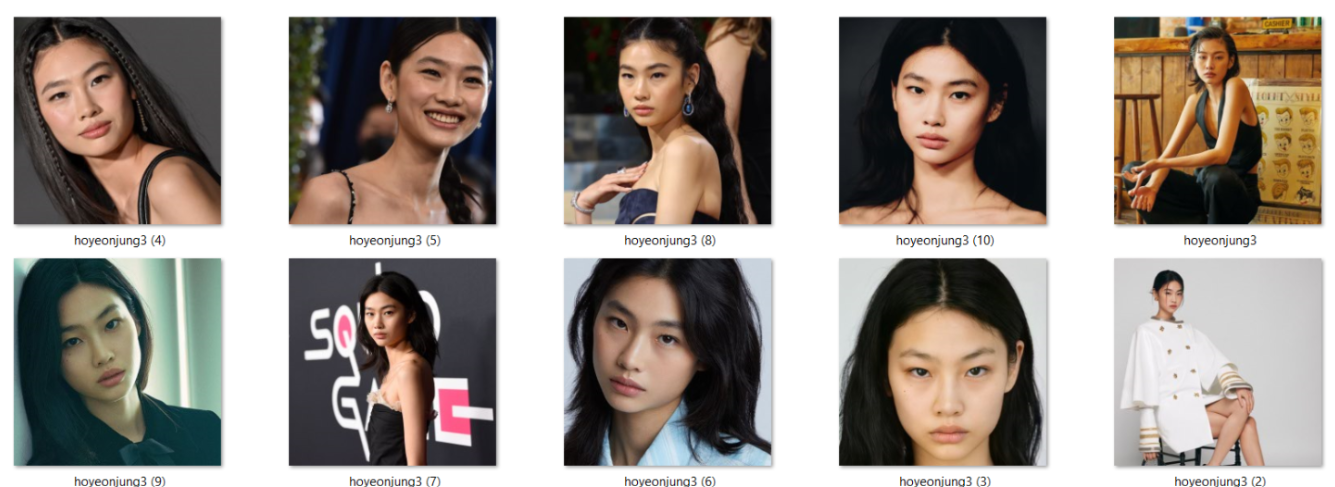
\includegraphics[width = 1
	\textwidth]{Imagenes/Vectorial/datasethoyeon.png}
	\caption{Dataset seleccionado para el entrenamiento de personas con Lora}
	\label{fig:datasethoyeon}
\end{figure}

Una vez que las imágenes cumplan con todos los requisitos, debemos utilizar el código abierto en la plataforma Google Colab para realizar el entrenamiento. 
El proceso que sigue el cuaderno es muy sencillo, en él sólo hace falta seguir una serie de pasos para completarlo. El primero es conectar el cuaderno a una cuenta de Google, para que se pueda guardar en el Drive asociado a esa cuenta una carpeta llamada ``Fast-Dreamboot'', en la que se guardaran todos los archivos que se generen durante el proceso. El siguiente paso es instalar las dependencias necesarias para ejecutar el código en python, seguido de establecer un nombre a la sesión en la que estamos trabajando, para que en un futuro cuando se hagan entrenamientos diferentes, se puedan distinguir unos de otros. En este paso se crea una carpeta llamada Sessions dentro de la carpeta mencionada recientemente. A su vez, esta carpeta contendrá otra bajo el nombre de la sesión que hayamos especificado en el cuaderno, y es ahí donde se guardaran todos los archivos que se creen en la ejecución. 

A continuación, es turno de subir las imágenes previa y cuidadosamente seleccionadas. Ya sea seleccionándolas directamente desde la carpeta en la que las tengamos guardadas en local, o habiéndolas subido previamente a una carpeta de la cuenta de Google Drive, y proporcionar la ruta en la que están en la celda del cuaderno habilitada para ello. 

El último paso, y uno de los más importantes, consiste en establecer algunos parámetros con los que se va a entrenar al modelo. El más importante y el único que nosotros hemos modificado, entre todos los que hay, es el número de steps. De modo que, en cuanto mayor sean, más tiempo tardará en generarse el archivo. Normalmente, se tardaba unos 20 o 25 minutos en terminar de entrenarse, lo cual hemos considerado que es bastante rápido. En el ejemplo de la figura \ref{fig:dreambooth} se puede ver la ejecución del progreso de entrenamiento en el que para una cantidad de 2000 pasos lleva 21 minutos y 36 segundos. 

Tras la finalización, se creará un archivo de alrededor de 2 giga bytes, que contendrá el modelo de Stable Diffusion 1.5, con una capa de entrenamiento más, puesto que incorporará el elemento deseado. Con esto ya tendríamos un elemento de inteligencia artificial personalizado.\\

\begin{figure}[h]
	\centering
	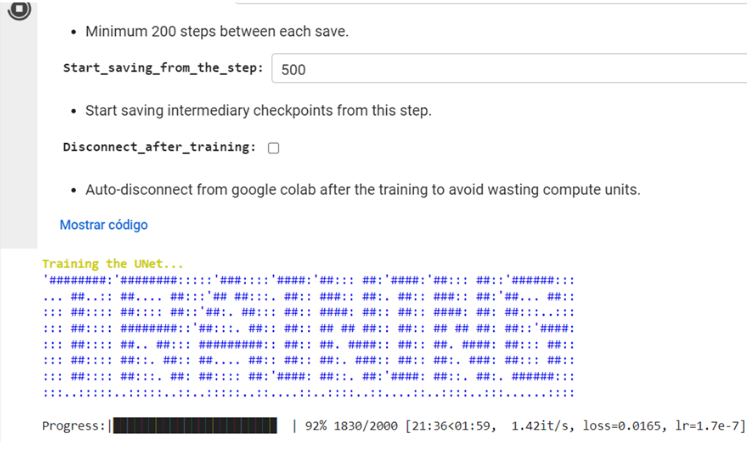
\includegraphics[width = 1
	\textwidth]{Imagenes/Vectorial/dreambooth.png}
	\caption{Procedimiento del entrenamiento mediante Dreambooth}
	\label{fig:dreambooth}
\end{figure}

Este archivo, en formato ckpt, se podrá utilizar en la aplicación NMKD SD GUI más adelante para generar imágenes, y contendrá el elemento entrenado bajo el token seleccionado. Si posteriormente se pretende incluir elementos al modelo ya entrenado, también se puede realizar empezando de nuevo el proceso de entrenamiento y utilizando de base el archivo en extensión ckpt anterior. Cuando se realice este segundo entrenamiento, se podrán generar imágenes acerca de ambos elementos, lo cuál es muy útil para nuestros objetivos, ya que en un mismo modelo enfocado a un paciente, debe haber múltiples elementos. Sin embargo, más adelante veremos que este último aspecto ha supuesto uno de los grandes fallos que experimenta el modelo en cuanto a múltiples capas de entrenamiento. \\

Un aspecto muy importante a tener en cuenta, es que tras la realización de múltiples pruebas, los resultados óptimos que hemos obtenido ha sido seleccionando un conjunto de datos formado por 10 imágenes, y con 2400 pasos de entrenamiento. 
%En la tabla \ref{tab:resultadosentrenamiento}\\



%\subsection{Entrenamiento con Dreambooth}
%\begin{table}
%	\centering
%	\begin{tabular}{c|c|c|c}
%		\textbf{Intento} & \textbf{Número de imágenes} & \textbf{Número de pasos} & \textbf{Veredicto} \\
%		\hline\hline
%		1 & 20 & 4000 & 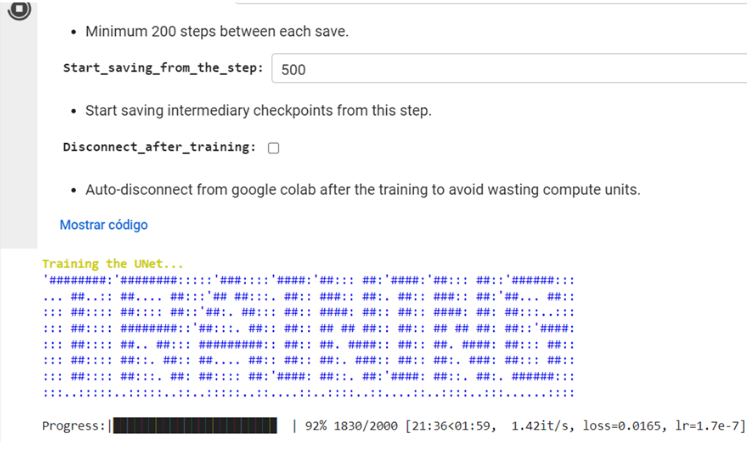
\includegraphics[width = 0.3
%			\textwidth]{Imagenes/Vectorial/dreambooth.png}\\
%		2 & 20 & 3000 & \\
%		3 & 15 & 3000 & \\
%		4 & 15 & 2000 & \\
%		5 & 10 & 3000 & \\
%		6 & 10 & 2400 & \\
%		\hline
%	\end{tabular}
%	\caption{Tabla de resultados obtenidos de entrenamiento}
%	\label{tab:resultadosentrenamiento}
%\end{table}


Hemos querido poner a prueba, no sólo las capacidades del modelo de entrenar a personas, ya que hemos podido comprobar sus puntos fuertes y débiles en la generación de seres humanos (los cuales podremos ver más adelante), sino de elementos que consideramos que también son de suma importancia a la hora de representar recuerdos: animales y lugares. \\

El objetivo de entrenar al modelo con lugares es que estos no se encuentren en la base de datos de imágenes de Stable Diffusion, puesto que de ser así, no tendría sentido realizar el entrenamiento. De este modo, podremos lograr que el paciente pueda rememorar sitios emblemáticos en su memoria y que las imágenes generadas que emulan recuerdos consigan ser aún más personales. Por ejemplo, el parque de su vecindario, la casa de sus padres o incluso, su propio salón. 

Las primeras pruebas que realizamos sobre un lugar se trataba de un edificio característico, que por supuesto no estaba incluido e el modelo previamente. Hablamos de la basílica de Colmenar Viejo, Madrid. Las imágenes seleccionadas estaban hechas desde diferentes ángulos, alturas, luces y lejanías. En la figura \ref{fig:datasetcolme} se pueden apreciar las características que reúnen las fotografías en cuestión y el token otorgado.

Además, quisimos comprobar si el número de imágenes y steps establecidos para las personas, producía resultados igual de satisfactorios para lugares. Y efectivamente, corroboramos la hipótesis de manera airosa. Ejemplos de ello, lo podemos ver en el apartado siguiente de Resultados.  

\begin{figure}[!htb]
	\centering
	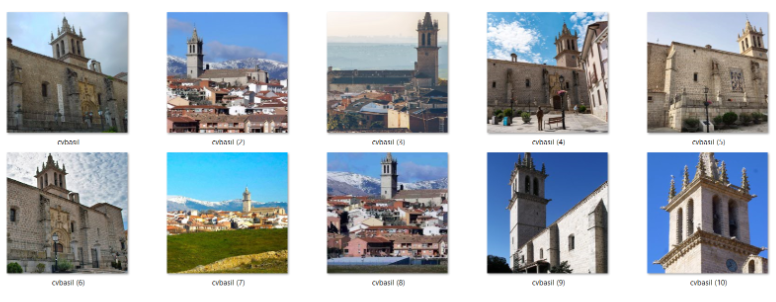
\includegraphics[width = 0.7
	\textwidth]{Imagenes/Vectorial/dataset_colmenar.png}
	\caption{Dataset seleccionado para el entrenamiento con lugares}
	\label{fig:datasetcolme}
\end{figure}


\subsection{Entrenamiento con la técnica de LORA}

Para el entrenamiento de animales, seleccionamos 10 fotografías de un perro de la raza Shiba Inu bajo diferentes perspectivas, escenarios y mostrando distintas expresiones para comprobar si la inteligencia artificial permitía entrenar con animales. Sin embargo, a la luz de los resultados vistos en personas y lugares quisimos comprobar la técnica de LORA que presenta Stable Diffusion. Las siglas LORA hacen referencia a \textit{Low-Rank Adaptation of Large Language Models}, del inglés. Esta técnica favorece un equilibrio entre el tamaño del archivo y la eficiencia del propio entrenamiento que ha presentado imágenes de gran calidad en un tiempo excepcional. 

En la figura \ref{fig:datasethachi} se pueden ver más en detalle las imágenes seleccionadas para las pruebas con LORA en animales.

\begin{figure}[h]
	\centering
	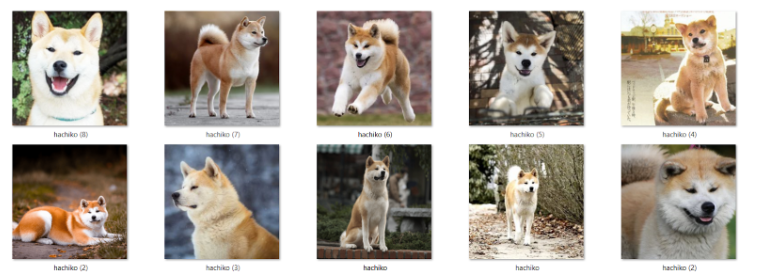
\includegraphics[width = 1
	\textwidth]{Imagenes/Vectorial/dataset_hachiko.png}
	\caption{Dataset seleccionado para el entrenamiento con animales}
	\label{fig:datasethachi}
\end{figure}

Como se puede apreciar en la figura anterior, se hizo hincapié en la diversidad de las imágenes, para aportar un mayor valor al entrenamiento, de modo que se tuviese una visión completa del elemento a entrenar.

Respecto al modo de ejecución, el hecho de cambiar a LORA no supuso grandes cambios a la hora de entrenar el elemento deseado debido a que la selección de imágenes es exactamente igual. Donde realmente cambia el entrenamiento es en el cuaderno utilizado en Google Colab, este es diferente y por lo tanto, la forma de ejecución y los pasos a seguir también lo son. 

Es de vital importancia saber cuáles son los parámetros que se deben ajustar para poder desarrollar el modelo de manera correcta y entender cada uno de ellos, dado que pueden resultar un poco más complejos en comparación con la técnica del cuaderno de Fast-Dreambooth.\\

El cuaderno de LORA de Google Colab, a diferencia del de Fast-Dreambooth, contiene una única celda de código con varios parámetros a ajustar y que  está ordenada en varias secciones. La primera sección es "Setup", lo que se puede traducir como la configuración o preparación, en ella se exige indicar el nombre del proyecto, la estructura de carpetas y por último, se debe especificar el modelo a entrenar entre tres opciones dadas (Anime, AnyLora y Stable Diffusion), y como se ha explicado anteriormente, hemos elegido el Stable Diffusion 1.5, al ser el que sirve de base para todos los entrenamientos escogidos. No obstante, esta técnica de entrenamiento tiene la peculiar característica de que se puede utilizar de base cualquier checkpoint desarrollado previamente, por lo que en caso de realizar un entrenamiento sobre personas, existe la posibilidad de elegir un modelo de base especializado en retratos. Esto garantiza que, seleccionando unas fotografías adecuadas y ajustando de manera correcta cada parámetro, los resultados sean bastante buenos.\\

La siguiente sección se llama "Processing", el parámetro más destacable en este apartado es la resolución de la imagen, a elegir entre 512, 640, 768, 896 y 1024. La elección dependerá del tamaño mínimo que tenga la imagen más pequeña de nuestro dataset.  En particular, y habiendo realizado múltiples entrenamientos con LoRA, cabe destacar que lo más recomendable es dejar la resolución de la imagen en 512 píxeles, es decir, tal y como aparece. Esto es porque aumenta considerablemente el tiempo de entrenamiento cuanto más alta es la resolución. Si se diera el caso de que esto provocase un aumento significativo en la calidad de las imágenes generadas, podría ser muy beneficioso. No obstante, entre una resolución de 512 y 1024 no se aprecia un gran salto de calidad, pero sí de tiempo, ya que aumenta desde los 20 minutos hasta más de una hora de tiempo de entrenamiento. Los demás parámetros son tags o etiquetas sobre la simetría y calidad de las imágenes. \\

Terminada esta, empieza la próxima sección ``Steps".
En cuanto a los steps de entrenamiento, en LoRA se deben indicar de un modo diferente, y aquí sí que presenta una gran ventaja respecto al modelo de Dreambooth. En este otro modelo, se indicaba un número concreto de pasos y como resultado, obteníamos un archivo en formato ckpt, de dos gigas de tamaño. Sin embargo, en LoRA se puede indicar un número de archivos que se deseen obtener. La peculiaridad de esto, es que cada número de pasos que se indique, se genera un resultado. De esta manera, en un mismo entrenamiento, se puede comprobar cuál es el número de pasos que genera la mejor fotografía. Este número de resultados se denomina \textit{epochs}, y en num repeats, se puede indicar el número de pasos que se entrenarán en cada \textit{epoch}. \\

\begin{figure}[h]
	\centering
	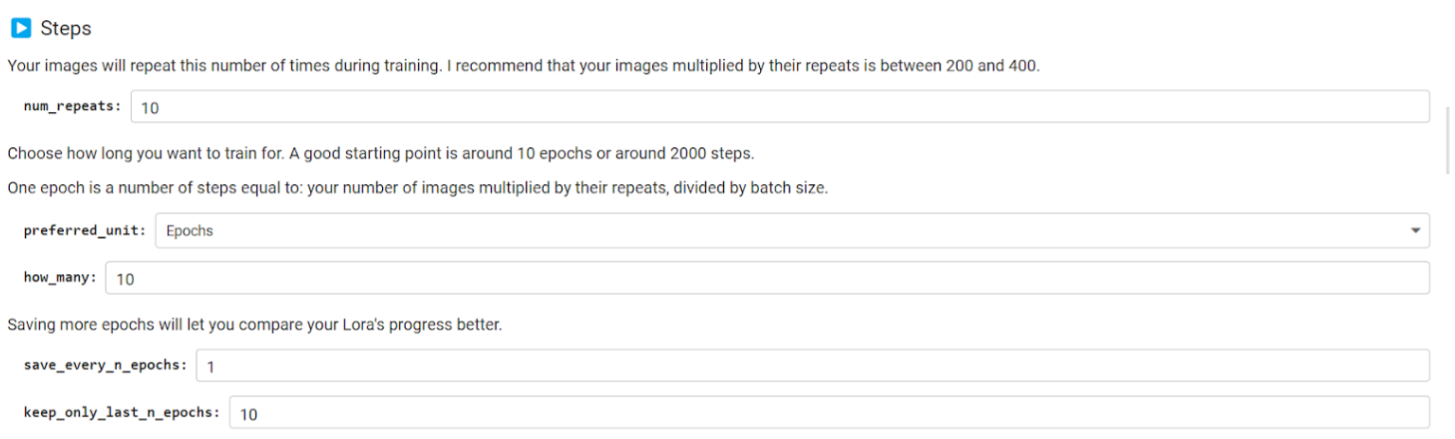
\includegraphics[width = 1.2
	\textwidth]{Imagenes/Vectorial/lora.png}
	\caption{Parámetros relevantes del entrenamiento con LoRA}
	\label{fig:lora}
\end{figure}

Por ejemplo, si se indica en este valor un 10, se obtendrá como resultado diez archivos en formato \textit{safetensor}. Estos archivos tienen un tamaño de alrededor de 18 MB, un tamaño mucho menor que un \textit{checkpoint}, de 2 GB. La diferencia reside en que el \textit{checkpoint} es un modelo nuevo a partir de uno pre entrenado, y el \textit{safetensor}, únicamente contiene el elemento que se ha entrenado, y para su ejecución necesita ir acompañado de su modelo de origen, en este caso el Stable Diffusion 1.5, lo que se ve reflejado en la siguiente imagen. De ahí nace la significativa diferencia de tamaño, por lo que, en cuanto a espacio de almacenamiento, es mejor la técnica de entrenamiento de LoRa. \\


Las secciones siguientes ``Learning'' de aprendizaje y ``Structure'' de estructura se refieren a variables que no se deben modificar del entrenamiento a cómo están preestablecidas, y por lo tanto, no hemos incidido en ellas.

Finalmente, la sección ``Ready'' nos indica que está ya todo listo para poder empezar el entrenamiento con LORA. \\

Ahora podemos decir que hemos logrado entrenar un modelo de generación de imágenes incluyendo fotografías propias, y eso es algo que puede ser realmente útil para nuestros siguientes propósitos. Esto es porque podemos lograr que cualquier persona pueda incorporar las imágenes que considere oportunas para servir de apoyo al paciente. Lo cual consideramos un éxito en el desarrollo de nuestro trabajo. 


\section{Interfaz de Stable Diffusion}

\subsection{Requisitos de instalación}

Respecto a los requisitos que debe cumplir un equipo para que pueda funcionar la aplicación NMKD Stable Diffusion GUI, es fundamental que tenga un mínimo de 8 GB de memoria RAM, siendo lo más recomendable que sea de 16 GB. También es muy importante el almacenamiento, donde además de tener un mínimo de 10 GB de espacio disponible, es conveniente que haya 5 GB extras, debido a que se van a guardar multitud de archivos temporales a medida que se utiliza la aplicación. Adicionalmente, para nuestro caso, que hemos utilizado la aplicación para comparar diferentes modelos, es necesario conocer que cada uno de ellos tiene un tamaño de alrededor de 5 GB, y los modelos entrenados derivados de Stable Diffusion ocupan 2 GB de almacenamiento cada uno. Por lo tanto, el espacio es algo que hay que tener muy en cuenta previamente a la instalación de este programa, ya que puede comprometer seriamente el funcionamiento del equipo. \\

La característica principal que debe cumplir un equipo y sin la cual no sería válido para utilizar la aplicación es el hecho de tener una tarjeta gráfica. Además, no sirve cualquier GPU, dado que el mínimo de memoria VRAM que debe tener el equipo es 4 GB, siendo la tarjeta de Nvidia. Más allá de que este sea el mínimo para que la aplicación funcione, a medida de que la tarjeta gráfica sea de mayor calidad y espacio, el rendimiento mejora exponencialmente. Para contextualizar, la tarjeta gráfica de nuestro equipo, una Nvidia GeForce GTX 1050, con una memoria de vídeo dedicada de 3072 MB y una memoria virtual disponible de 8 GB, tarda alrededor de varios minutos en generar una fotografía con cierta calidad. Mientras tanto, tarjetas gráficas como la RTX 4090, genera las imágenes en 1 segundo, lo cual es bastante significativo. No obstante, esta tarjeta tiene un precio en el mercado de alrededor de 2000 euros, por lo que en nuestro nivel, mejorar el rendimiento es algo que se antoja complicado, y que la duración que va a tener nuestro proceso de generación de imágenes será siempre de varios minutos.\\


\subsection{Funcionamiento y detalles de la interfaz}

 Respecto al funcionamiento de SDGUI, esta plataforma tiene una interfaz muy sencilla para el usuario, a pesar de que hay que tener conocimientos previos acerca de ciertos parámetros para poder llevar a cabo la generación de de imágenes, además de realizar múltiples pruebas para saber qué función cumple cada elemento. La aplicación se presenta tal y como aparece en la siguiente imagen, y permite generar imágenes con modelos de Stable Diffusion, con modelos obtenidos de Hugging Face, con modelos entrenados y con LoRA. Esto ofrece una gran ventaja para nuestro trabajo, ya que ha sido el programa que nos ha permitido probar qué modelo era el más adecuado para nuestro estudio, y posteriormente testar los entrenamientos realizados. Ha sido fundamental, porque han sido miles de pruebas, ajustando todos los parámetros de múltiples maneras diferentes, y sin esta aplicación, avanzar y obtener resultados habría sido realmente complicado. Respecto a la estructura del programa, cuenta con una parte derecha de la pantalla, donde aparecen las imágenes generadas en un gran recuadro, se puede acceder a un historial de descripciones introducidas y se puede acceder a una carpeta que incluye todas las imágenes que han sido generadas por esta aplicación. Además, en la parte superior, se puede acceder a ajustes, donde es posible instalar nuevas versiones del programa u obtener nuevos modelos que poder utilizar para la generación de imágenes. \\
 
 
 \begin{figure}[h]
 	\centering
 	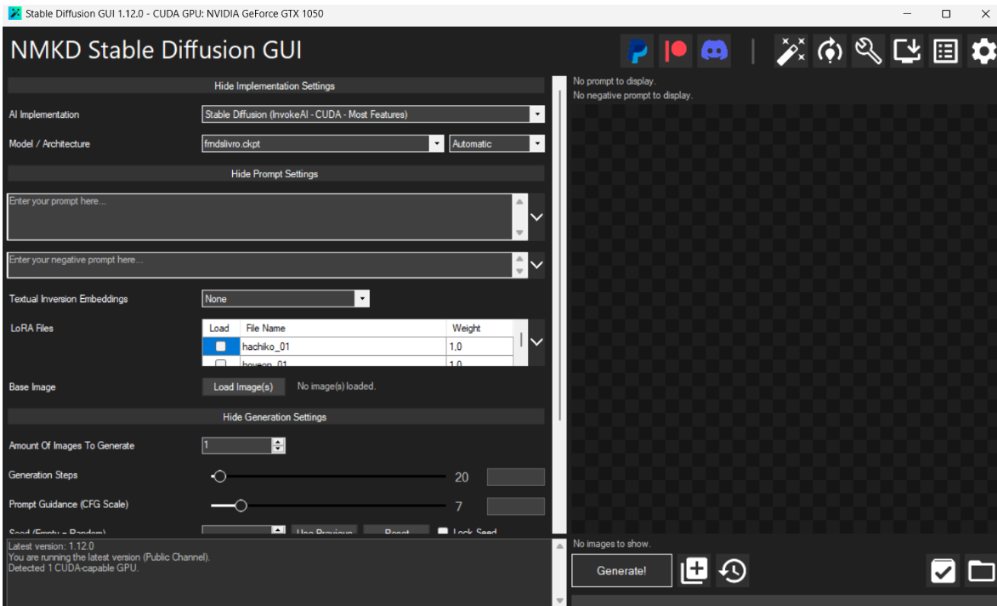
\includegraphics[width = 1
 	\textwidth]{Imagenes/Vectorial/nmkdsdgui.png}
 	\caption{Aplicación SDGUI, utilizada para probar todos los modelos generadores de imágenes }
 	\label{fig:nmkdsdgui}
 \end{figure}
 
 En la parte izquierda de la pantalla, podemos encontrar los parámetros realmente importantes que condicionan la manera en la que se creará la siguiente fotografía. En primer lugar, el tipo de inteligencia artificial utilizada. Esto es realmente relevante porque hace una distinción de cuatro tipos de IA generativa: dos son versiones estándar de Stable Diffusion (una para los sistemas que utilicen CUDA o Nvidia, y otra para los que utilicen AMD como tarjeta gráfica), la tercera es la versión XL de Stable Diffusion, que como recordatorio, requiere una tarjeta gráfica muy superior a la que dispone nuestro equipo, y por último, un modelo imagen a imagen. Resulta muy relevante hablar sobre esta IA, dado que a partir de una imagen de archivo, y una descripción, se puede generar una nueva imagen adaptada a esta petición. A pesar de que nuestro objeto de estudio abarca la inteligencia artificial generativa de imágenes a partir de texto, hemos realizado pruebas sobre el tipo de resultado obtenido, pero la calidad de la imagen de este modelo en concreto, resulta inferior a la que nos han otorgado modelos de texto a imagen. Centrándonos en el modelo básico de Stable Diffusion, en el apartado de \textit{model} / \textit{architecture}, se debe incluir el modelo, que puede ser uno pre entrenado o uno personalizado en formato \textit{checkpoint}. En este segundo, cabe destacar que tarda medio minuto más en generar la fotografía debido a la carga, pero no afecta de ninguna manera a la calidad de la imagen. \\
 
 A continuación, se debe indicar la descripción, que se divide en dos partes en este caso. La primera es el \textit{prompt}, que guía a la inteligencia artificial para que incluya los elementos que se deseen. Un apunte relevante es que si se quiere hacer referencia a un elemento entrenado, se debe mencionar el nombre exacto del ítem para que se pueda realizar la generación de manera correcta. En segundo lugar, existe un \textit{negative prompt}, donde se deben indicar aquellos elementos que, a petición del usuario, se desee que no se vean reflejados en la creación de la fotografía. Cuando se desee testar un entrenamiento de LoRA, se debe hacer click en el archivo deseado, e introducir ese nombre en el \textit{prompt}. Por último, se deben ajustar unos parámetros explicados con anterioridad, como son los \textit{steps} o pasos de generación, la escala CFG y la \textit{seed}. Una vez conocidos estos pasos a seguir y cumplidos los requisitos mencionados, cualquier usuario debería tener la capacidad de generar imágenes mediante inteligencia artificial con este programa.\\

\section{Resultados de generación de imágenes}

Visto el funcionamiento de la aplicación, vamos a analizar los resultados obtenidos en comparación con los \textit{prompts} especificados y bajo las posibles diferentes técnicas y parámetros que se han contemplado. 


\subsection{Resultados con personas}
Una buena manera de mostrar el mejor resultado posible de una generación de imágenes personalizadas es estudiar cuál es el método que genera mejores fotografías. Para ello, hemos realizado un análisis comparativo de resultados con diferentes pasos de entrenamiento.

El objetivo es comprobar cuál es el número de pasos del entrenamiento mediante Dreambooth que genera las imágenes con mayor calidad y precisión posible. Para ello, hemos realizado cuatro entrenamientos del mismo elemento, con el mismo \textit{dataset} de 10 fotografías, pero con un número de pasos diferente. Este número ha sido de 1600, 2000, 2400 y 3000 \textit{steps}. El tiempo de generación aproximada es de 1,38 iteraciones por segundo, lo cual conlleva una duración total de entrenamiento de 19, 24, 29 y 35 minutos aproximadamente, y es algo a tener en cuenta para seleccionar un modelo u otro.\\

Para poder llegar a resultados concluyentes, se han de fijar todas las variables de la generación de imágenes en la aplicación SDGUI. Estas variables son la descripción de la fotografía, los pasos de generación, la escala CFG y la semilla de aleatoriedad. De esta manera, se tiene la capacidad de realizar una comparación precisa y de elegir el número más adecuado de pasos de entrenamiento. En este caso, dada nuestra experiencia al generar imágenes con Stable Diffusion, establecimos el número de pasos en 20 y la escala CFG en 7. Respecto a la semilla de aleatoriedad, tras la primera fotografía generada se fijaría para el resto, para que permanezca constante en nuestro análisis.\\

Hemos optado por utilizar varios tipos de fotografía diferente para poder ampliar la calidad de la conclusión. La primera descripción de imagen trataba de generar un retrato de la persona lo más detallado posible, de manera que se pudiera comparar con qué pasos la capacidad de identificar al elemento entrenado era mayor. Con el segundo \textit{prompt}, se pretendía analizar la generación de las imágenes de la persona haciendo una acción determinada. En este caso, se optó por la lectura de un libro. De este modo, se podría afirmar cuál de los modelos tendría la capacidad de generar fotografías personalizadas de múltiples elementos, lo cual es algo bastante relevante para nuestro trabajo. Por tanto, en la siguiente tabla se refleja la imagen generada con cada número de pasos de entrenamiento, con las dos descripciones mencionadas.\\

 \begin{table}
	\centering
	\begin{tabular}{>{\centering\arraybackslash}m{5cm} >{\arraybackslash}m{5cm}>{\arraybackslash}m{5cm}}
		\textbf{Pasos de entrenamiento} & \textbf{\textit{a portrait of 80alp, highly detailed, happy, old}} & \textbf{\textit{a picture of 80alp reading a book, serious, high definition}} \\
		\hline
		1600 & 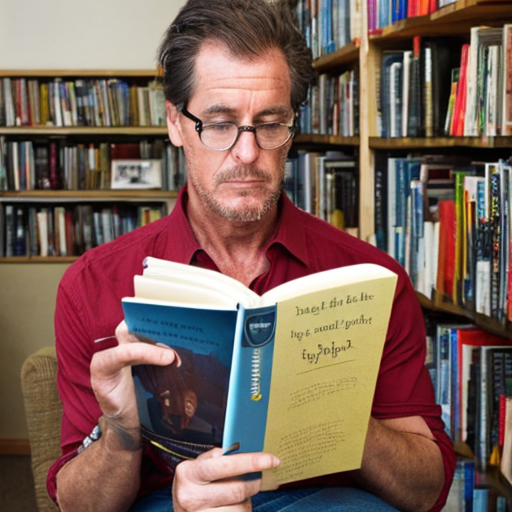
\includegraphics[width = 0.3
		\textwidth]{Imagenes/Vectorial/80alp1600.png & \includegraphics[width = 0.3
		\textwidth]{Imagenes/Vectorial/1600pasosbook.png}\\
		\hline
		2000 & 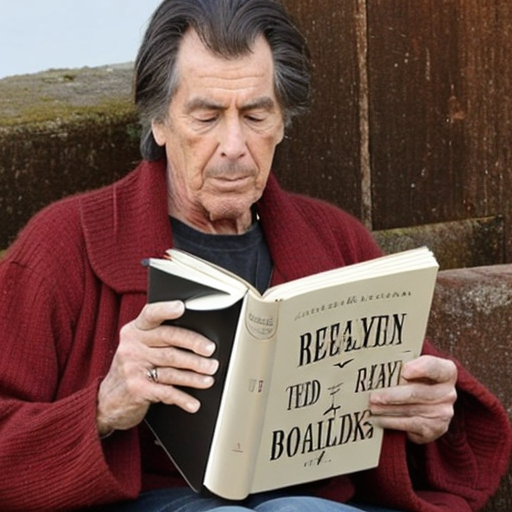
\includegraphics[width = 0.3
		\textwidth]{Imagenes/Vectorial/80alp2000.png & \includegraphics[width = 0.3
		\textwidth]{Imagenes/Vectorial/2000pasosbook.png}\\
		\hline
		2400 & 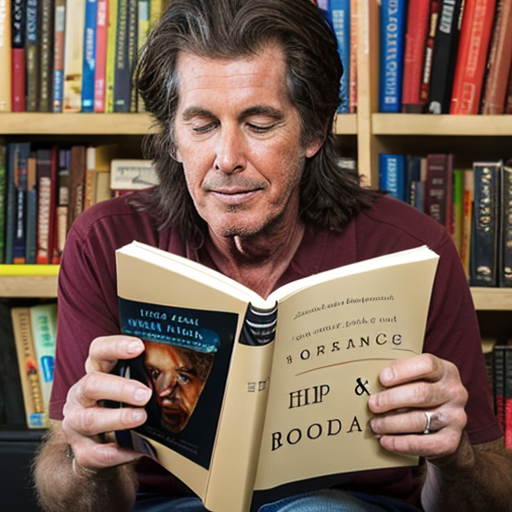
\includegraphics[width = 0.3
		\textwidth]{Imagenes/Vectorial/80alp2400.png & \includegraphics[width = 0.3
		\textwidth]{Imagenes/Vectorial/2400pasosbook.png}\\
		\hline
		3000 & 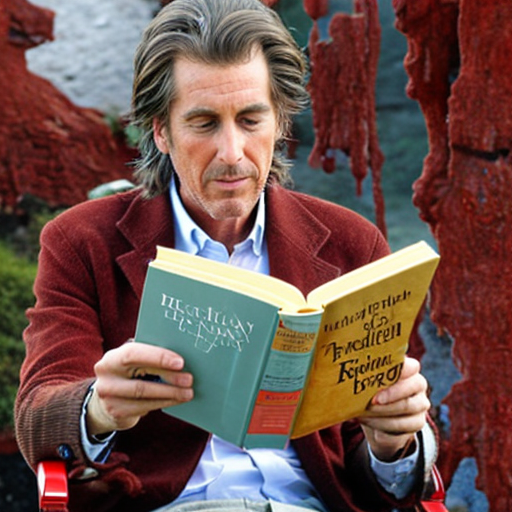
\includegraphics[width = 0.3
		\textwidth]{Imagenes/Vectorial/80alp3000.png & \includegraphics[width = 0.3
		\textwidth]{Imagenes/Vectorial/3000pasosbook.png}\\
		\hline
	\end{tabular}
	\caption{Tabla de resultados obtenidos del Capítulo 1 de juventud del paciente}
	\label{tab:capitulo1librovida}
\end{table}


Tras generar todas las fotografías, en primer lugar, se aprecia falta de entrenamiento en las dos imágenes con 1600 \textit{steps}, debido a que no se identifica bien a la persona, ni en el retrato, ni en la imagen con el libro. En la primera fotografía se puede observar una gran calidad, con mucho detalle y un ligero parecido con la persona entrenada, pero no es el nivel de similaridad que estamos buscando. En la imagen con el libro, la persona generada no se puede identificar con la real, y, además de eso, se aprecia deformidad en las manos, por lo que la fotografía generada no tiene el nivel de calidad deseado. \\

En segundo lugar, al incrementar los \textit{steps} de entrenamiento a 2000, se puede apreciar una clara mejoría. En el retrato, existe un gran parecido con la imagen generada con 1600 pasos, pero se aprecia como la forma de la cara se asemeja más a la persona real. Respecto a la fotografía con el libro, en esta ocasión se han solucionado los errores de deformidad, y se ha generado a una persona de la edad correspondiente, aunque no se puede identificar a la persona real.\\

Con 2400 pasos de entrenamiento, se puede decir que los resultados muestran calidad. En la primera fotografía, se puede identificar un gran parecido con la persona real. La imagen muestra un gran detalle y una definición muy buena, por lo que mejora en gran medida a los números de pasos menores. En la segunda fotografía, existe cierto parecido con la persona, pero se puede mejorar, debido a que falta detalle y definición y se muestra a alguien mucho más joven. A pesar de esto, sí que la forma de la cabeza y de la cara parecen ser correctas, por lo que lo único que faltaría para que la generación fuera adecuada es la edad, lo cual se podría arreglar con una descripción más precisa.\\

Al incrementar los \textit{steps} a 3000, se puede apreciar sobreentrenamiento, debido a que en ambas imágenes se ha perdido el parecido con la persona real y se puede percibir algo de deformidad, sobre todo en la segunda fotografía. Respecto al retrato, ha variado la forma y el color de los ojos, y han aparecido más marcas que empeoran la calidad. En la imagen con el libro, se ha generado a una persona aún más joven que con 2400 pasos, y ha cambiado por completo la forma de la cara, por lo que la similitud con la persona real se ha desvanecido por completo. Además, si se amplía en detalle se puede apreciar deformidad en los ojos, por lo que se hace evidente el sobreentrenamiento. \\

En conclusión, podemos decir que el entrenamiento que ha producido mejores resultados es el de 2400 pasos, que con menos se aprecia falta de entrenamiento y que con más \textit{steps} se percibe sobreentrenamiento y no se permite identificar a la persona real. En este estudio también se ha podido aprender que el prompt ha de ser lo más preciso posible para poder obtener imágenes de gran calidad, sobre todo cuando se trata de incluir más elementos. En este caso, la escala CFG debería ser mayor, para dar algo menos de libertad al modelo y que se centre más en lo que se pide en la descripción.


\begin{figure}[!htb]
	\centering
	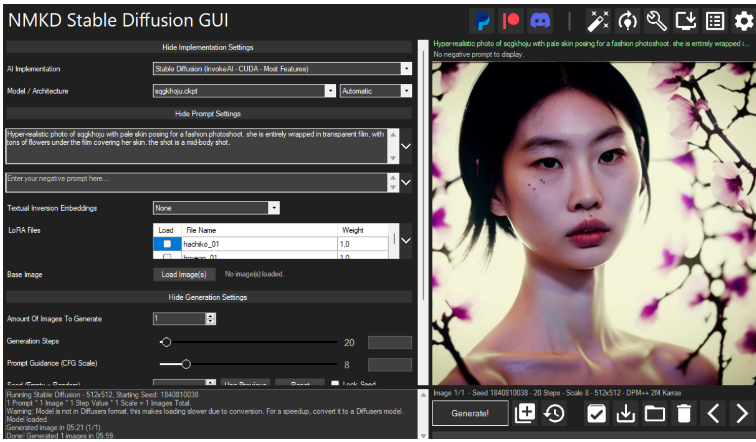
\includegraphics[width = 1
	\textwidth]{Imagenes/Vectorial/hoyeon1.png}
	\caption{Resultados de entrenamiento de una persona con Dreambooth}
	\label{fig:hoyeonsd}
\end{figure}

que tallll\\

\begin{figure}[!htb]
	\centering
	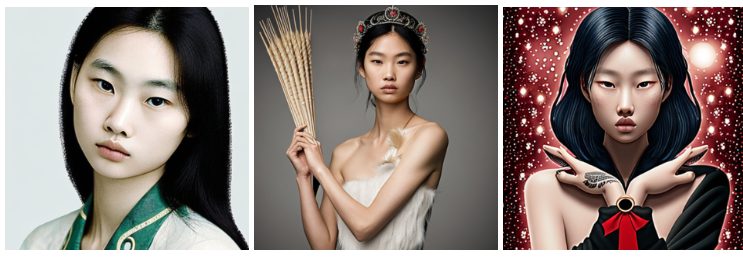
\includegraphics[width = 1
	\textwidth]{Imagenes/Vectorial/hoyeon_results.png}
	\caption{Resultados de entrenamiento de una persona con diferentes estilos}
	\label{fig:imagshoyeon}
\end{figure}

\subsection{Resultados con lugares}

Con diferentes estilos:\\

\begin{figure}[!htb]
	\centering
	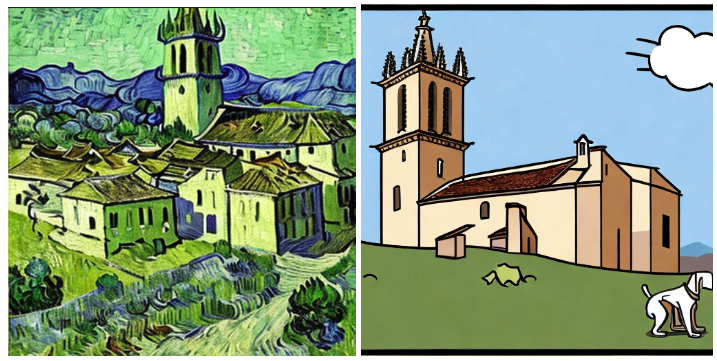
\includegraphics[width = 1
	\textwidth]{Imagenes/Vectorial/colmenar_styles.png}
	\caption{Resultados de imagenes del lugar entrenado al estilo Van Gogh y viñeta}
	\label{fig:colmestyles}
\end{figure}


Añadiendo otros elementos:\\


\begin{figure}[!htb]
	\centering
	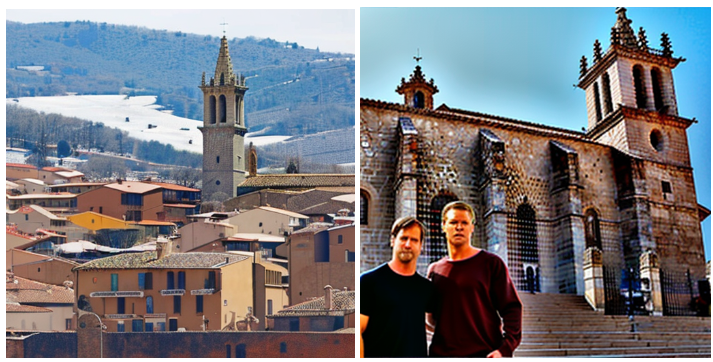
\includegraphics[width = 1
	\textwidth]{Imagenes/Vectorial/colmenar_elements.png}
	\caption{Resultados de imágenes del lugar en invierno y con una persona}
	\label{fig:elementscolme}
\end{figure}

\subsection{Resultados con animales}
hellloouuuuu\\

\begin{figure}[!htb]
	\centering
	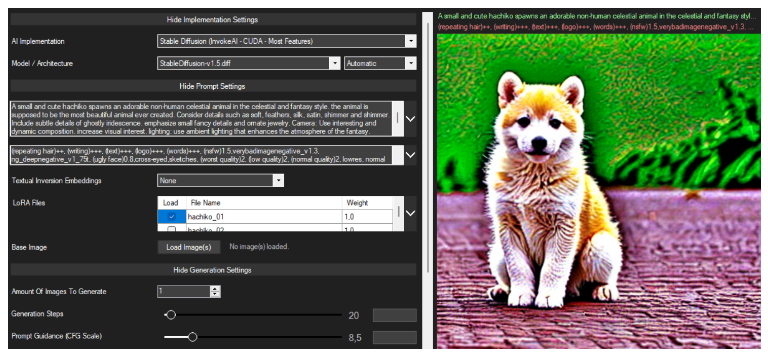
\includegraphics[width = 1
	\textwidth]{Imagenes/Vectorial/hachiko_detallada.png}
	\caption{Imagen generada con el modelo Stable Diffusion 1.5, Lora Hachiko}
	\label{fig:detallehachi}
\end{figure}

heyyyyy\\

\begin{figure}[!htb]
	\centering
	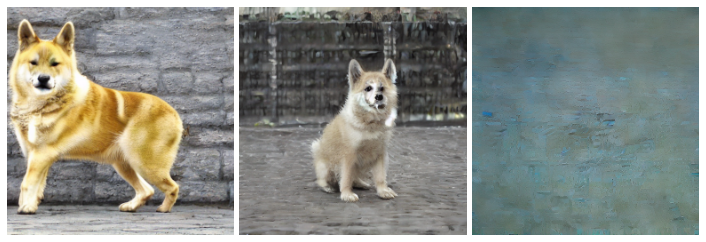
\includegraphics[width = 1
	\textwidth]{Imagenes/Vectorial/comparacion_hachiko.png}
	\caption{Mismo prompt con 1000, 2000 y 10.000 pasos de entrenamiento}
	\label{fig:comphachi}
\end{figure}

\subsection{Resultados con múltiples capas de entrenamiento}

Una parte muy importante de nuestro trabajo es generar imágenes que puedan contener diferentes elementos de manera simultánea, puesto que consideramos que para crear un libro de vida de calidad, se deberían incluir fotografías de una persona en un determinado lugar, o que combinen varias personas diferentes. Durante la mayor parte del tiempo en la que realizamos este proyecto, teníamos la idea de que esto no sería posible, porque siempre que realizábamos pruebas, obteníamos resultados en los que se deformaban los elementos, o simplemente solo incluía uno de los dos elementos, o ninguno de los dos. 

A pesar de esto, decidimos resistirnos a aceptar que no podía ser posible una generación de imágenes en la que se combinasen varios elementos. Como hemos afirmado en apartados anteriores, nuestro modelo de entrenamiento Dreambooth permite realizar un entrenamiento sobre otro previo, por lo que decidimos hacer la prueba y añadir una capa. Para el entrenamiento, utilizamos como base el archivo sqgkhoju.ckpt, el cual entrenó a la actriz Jung Hoyeon, y se entrenó con el salón de la serie \textit{Friends}. Como en el resto de pruebas con las que obtuvimos un resultado satisfactorio, incluimos un conjunto de 10 imágenes y realizamos el entrenamiento con 2400 pasos.\\

\begin{figure}[!htb]
	\centering
	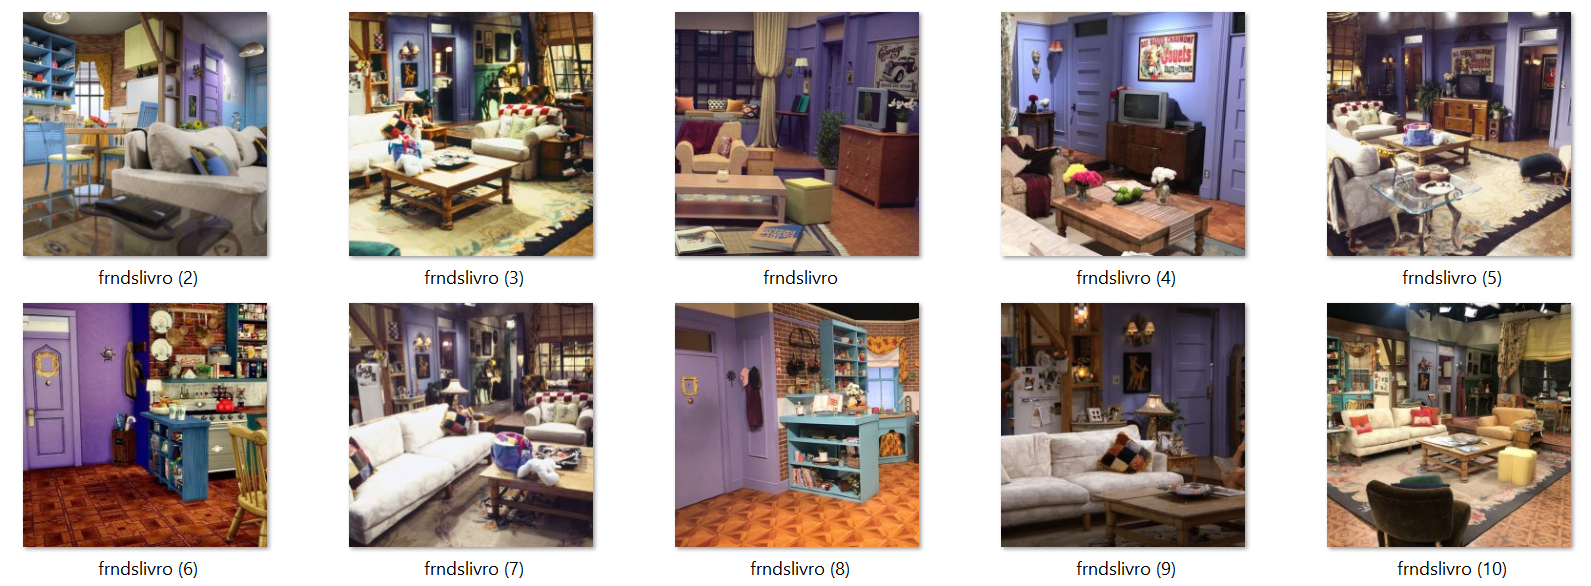
\includegraphics[width = 1
	\textwidth]{Imagenes/Vectorial/dataset_frdslivro.png}
	\caption{Dataset del entrenamiento con el salón de Friends (frndslivro)}
	\label{fig:dataset_frdslivro}
\end{figure}


Una vez realizado el entrenamiento, en primer lugar, se comprobó que se podían generar buenas fotografías que incluyesen únicamente el salón, antes de crear imágenes con ambos elementos.\\

\begin{figure}[!htb]
	\centering
	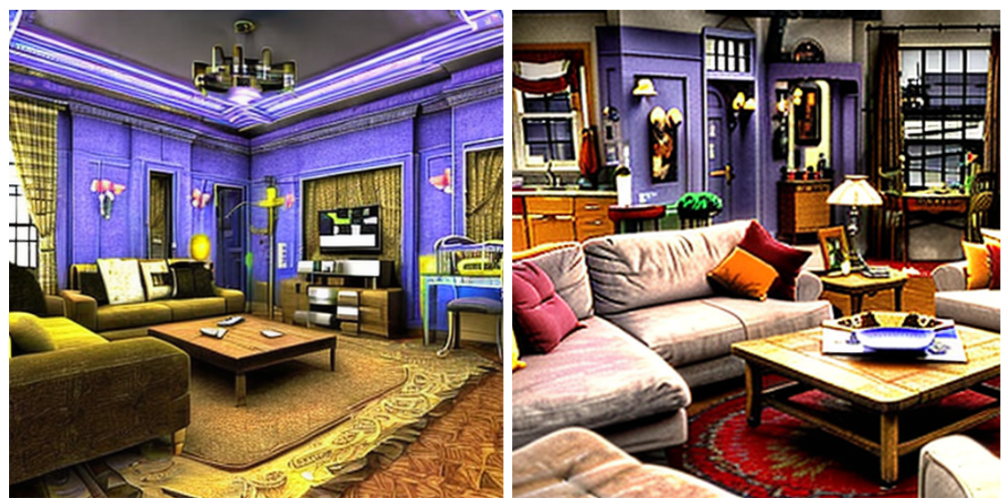
\includegraphics[width = 1
	\textwidth]{Imagenes/Vectorial/resultadosfrndslivro.png}
	\caption{Resultados de la generación de imágenes con el modelo ``frndslivro''}
	\label{fig:resultsfrnds}
\end{figure}

Como se puede apreciar, las imágenes generadas son de calidad, están creadas con 20 pasos de generación, 8 de \textit{CFG scale} y con diferentes estilos. Viendo que el modelo genera las fotografías de manera exitosa, es el momento de crear imágenes de la persona en el salón. Siguiendo la tendencia de 20 pasos y 8 de CFG, se producían errores en la generación, creándose imágenes en las que aparecía la persona duplicada y no aparecía el lugar. Ateniéndonos a la definición de \textit{CFG scale}, subimos este valor, de 8 a 14, para que la inteligencia artificial se guiase en mayor medida por el \textit{prompt}. Con solo subir este valor no fue suficiente, pues generaba fotografías en las que la persona aparecía entre 3 y 4 veces. Por tanto, también decidimos aumentar los pasos de generación, de manera sucesiva hasta que la generación produjera un resultado satisfactorio. La combinación perfecta fue de 40 pasos y 14,5 de \textit{CFG scale}. Con un número menor de \textit{steps}, la imagen aparecía con múltiples personas, y con un número mayor, no generaba ninguna persona. La descripción de la imagen era la siguiente: a ``sqgkhoju in the frndslivro, hd, high quality''.\\

\begin{figure}[!htb]
	\centering
	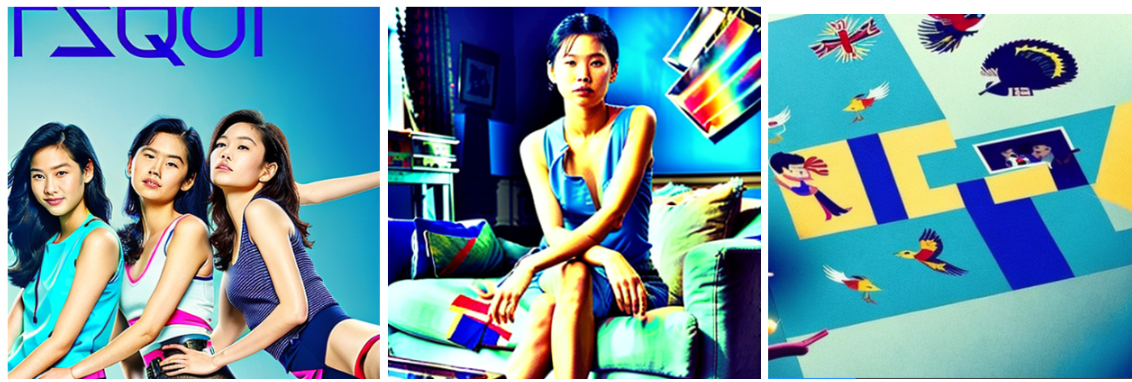
\includegraphics[width = 1
	\textwidth]{Imagenes/Vectorial/resultadoshojuyfrnds.png}
	\caption{Mismo prompt con 20, 40 y 50 steps al mezclar dos elementos: persona y lugar}
	\label{fig:comphachi}
\end{figure}


\subsection{Logros y fallos en resultados}

A lo largo de la variedad de entrenamientos realizados hemos hecho pruebas exhaustivas sobre la generación de las imágenes en comparación con los \textit{prompts} especificados y hemos sacado en claro que hay 3 aspectos fundamentales que hay que tener en cuenta para la generación óptima de estas: el número de pasos realizados en el entrenamiento, en el número de pasos para la generación de la foto y la escala CFG. 

En los tres aspectos, hemos identificado dos posibles situaciones que se pueden dar y que presentan fallos en cuanto a la calidad de los resultados: exceso y falta de pasos en el entrenamiento. 


- Peligros con el sobreentrenamiento: Se produce cuando el modelo no se puede generalizar y se ajusta demasiado al conjunto de datos entrenados. Se debe principalmente a que el tamaño de los datos es demasiado pequeño y no contiene suficientes muestras de datos para poder representar con precisión la totalidad de datos de entrada posibles. Otra razón es que el modelo se entrena durante demasiado tiempo en un solo conjunto de datos de muestra. En nuestro modelo, encontramos sobreentrenamiento cuando elegimos un número de \textit{steps} muy elevado para un número de fotografías que no es lo suficientemente alto. Una manera de detectar que nuestro modelo está sobreentrenado es cuando no genera bien la cara de la persona, y se aprecian fallos en determinadas facciones, como en los ojos y la boca, en los cuales se aprecia deformidad.\\

- Falta de pasos en el entrenamiento: En este caso, se produce cuando el modelo de datos no tiene la capacidad de capturar de forma precisa la relación entre las variables de entrada y de salida, de manera que existe un elevado índice de errores en el conjunto de datos de entrenamiento y en los datos no vistos. Se debe a que el modelo es demasiado simple, porque el tamaño de los datos es demasiado pequeño, o bien porque se necesita más tiempo de entrenamiento. En este caso, cuando generamos las imágenes, se evidencia que el modelo aún no ha aprendido lo suficiente acerca del elemento o \textit{token} del que se ha realizado el entrenamiento, pues el resultado de la generación refleja una persona que no muestra ningún parecido con la realidad.\\


En cuanto a mezcla de personas: Para ampliar los horizontes de nuestro entrenamiento, hemos entrenado a una persona, asociando un \textit{token} a ella para su identificación, sobre un modelo que previamente ya había sido entrenado con una persona y su \textit{token} asociado, para comprobar si efectivamente se podía generar en una sola imagen una representación de las dos personas entrenadas, una junto a la otra. Es aquí donde se ha detectado una peculiaridad, ya que, a pesar de que un modelo genere buenos resultados de cada una de las dos personas, en el mismo momento que se solicita en un determinado \textit{prompt} o descripción que se vean reflejados una o varias personas entrenadas en la misma fotografía, ningún modelo de los que se haya probado, ha generado buenos resultados de esta manera. Lo que finalmente se aprecia en la imagen generada, es que aparecen dos personas pero sus rostros son una mezcla de las características faciales y fisiológicas de ambas, produciéndose una deformidad en muchos de los casos y que los rostros aparezcan prácticamente duplicados.


\begin{figure}[h]
	\centering
	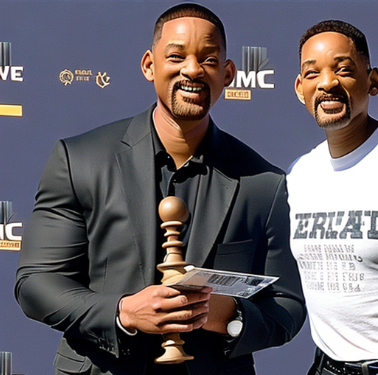
\includegraphics[width = 0.5
	\textwidth]{Imagenes/Vectorial/duplicidad_will.png}
		\caption{Duplicidad de elementos}
	\label{fig:willpor2}
\end{figure}

\subsection{Soluciones: Técnica \textit{Inpainting}}

Debido a la importancia que consideramos que tiene en el desarrollo de unas adecuadas historias de vida la mezcla de elementos personales con la propia persona, consideramos métodos para arreglar la poca certeza que nos otorga el modelo de Stable Diffusion con múltiples capas de entrenamiento, ya que a la luz de los resultados, el modelo es, por el momento, inválido en este aspecto. \\

Por ello, decidimos profundizar en las opciones que ofrece la interfaz de Stable Diffusion y dimos con la opción img2img, es decir, imagen a imagen. Esto es, como su nombre indica, un método en el que la entrada, en vez de ser texto como lo venía siendo hasta ahora, es una propia imagen. Sin embargo, el \textit{prompt} sigue siendo un elemento fundamental que sigue formando parte del modelo, ya que de esta manera, se le especifica a la Inteligencia Artificial lo que se desea en la imagen futura y el modelo se encargará de crearlo, teniendo en cuenta la estructura y objetos ya dispuestos en la imagen original. 

Incluso, el propio modelo de Stable Diffusion con el método de img2img tiene sus propias técnicas, de las cuales, una particularmente llamó nuestra atención: la técnica \textit{Inpainting}. 

Entre los problemas que se encontraban en el contenido final de las imágenes pedidas bajo un \textit{prompt} que integraba dos elementos entrenados, podíamos distinguir 3 casos principales: contenido aleatorio no especificado, falta completa de uno de los dos elementos o un elemento y el concepto del segundo elemento sin llegar a ser el propio. 

Por tanto, podemos llegar a afirmar que el último caso es el que más se asemejaba a lo que queríamos llegar a conseguir. Por ejemplo, si en el \textit{prompt} especificábamos que apareciera el \textit{token} que se asocia a una persona entrenada junto al \textit{token} asociado a un animal entrenado, la gran mayoría de los resultados era el perro entrenado a la perfección junto a una persona que no se asemejaba de ninguna manera a la entrenada.  

Lo que nos llegó a pensar que realmente la imagen generada de por sí, no era del todo errónea, ya que tan solo necesitábamos cambiar una pequeña porción de la misma: la persona de la imagen por la entrenada por nosotros en el modelo. Y es precisamente lo que logra la técnica de \textit{inpainting}. 

Esta novedosa técnica debe su nombre a que el protagonista es un pincel virtual. Para ejecutarla, necesitamos como entrada una imagen, en nuestro caso, la imagen recién generada por el modelo que presenta una carencia. Con el pincel, dibujamos el área de la imagen que deseamos sustituir por otro elemento. Y a través del \textit{prompt}, especificamos aquello que solamente queremos que aparezca en el área trazada, en este caso, el \textit{token} que representa a la persona entrenada. 

De esta manera, la Inteligencia artificial genera lo especificado en el \textit{prompt} solamente en el área indicada sustituyéndolo por lo que había anteriormente. En este ejemplo, el área que dibujaríamos correspondería a la persona de la foto y el resultado final serían los dos elementos diferentes integrados a la perfección en una sola imagen. 

Debido a la novedad de la técnica, los parámetros que estábamos acostumbrados a cambiar, también se han ampliado para poder emplear la técnica con los mejores resultados posibles y de la manera más eficiente. 

Entre ellos, los más importantes y que se pueden ver en la figura \ref{fig:paramsinpainting} señalados, son 5, con los cuales dos ya estamos familiarizados, que son los \textit{steps} y \textit{cfg scale}. Por lo tanto, nos centraremos más en los 3 restantes. 

\begin{figure}[h]
	\centering
	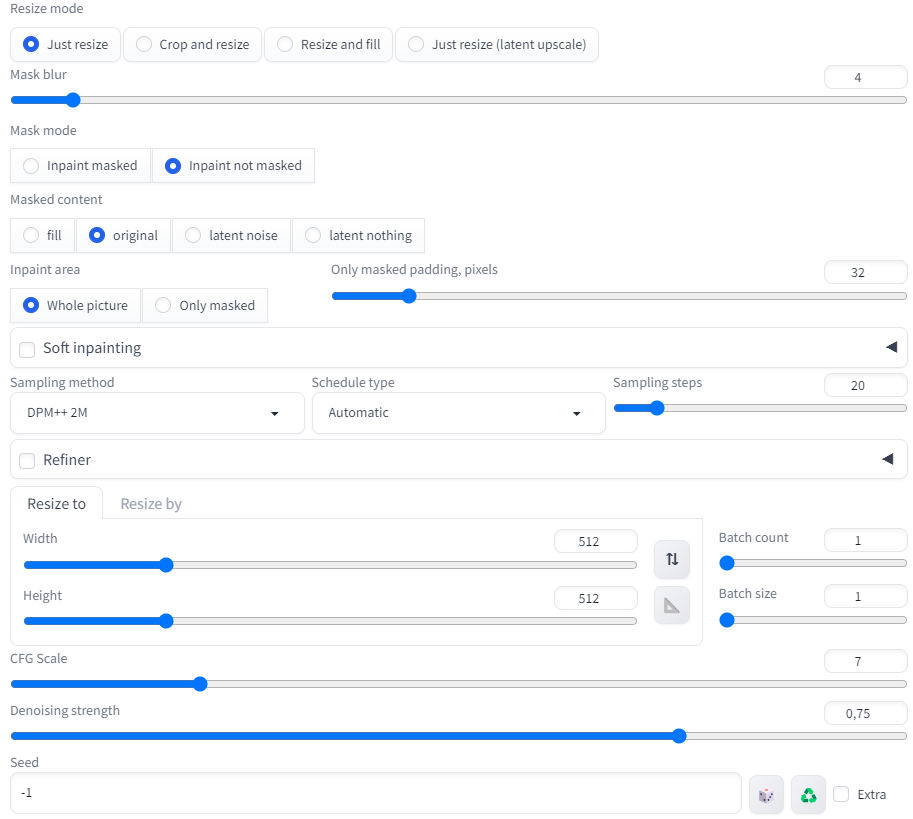
\includegraphics[width = 0.6
	\textwidth]{Imagenes/Vectorial/parametrosinpainting.png}
	\caption{Configuración de los parámetros en la técnica de inpainting}
	\label{fig:paramsinpainting}
\end{figure}

El primer parámetro es ``\textit{Mask Mode}'' y antes de continuar, es importante especificar que en \textit{Inpainting}, cuando se habla de ``\textit{mask}'' se refiere únicamente al área que hemos marcado con el pincel para su posterior modificación. Como podemos ver en la figura \ref{fig:gan}, en este parámetro se encuentran dos opciones: \textit{inpaint masked} e \textit{inpaint not masked}. A lo que se refiere es al área que se va a ver sustuida por el \textit{prompt}, ya que habrá casos en los que se quiera conservar la imagen en su totalidad a excepción de una parte y casos que por el contrario, se desearía modificar la imagen en su totalidad, a excepción de una porción, como lo puede ser en el caso de un cambio de fondo. 

El segundo parámetro es ``\textit{Masked content}'' y las opciones que presenta son un poco más extensas que en el parámetro anterior, siendo estas \textit{fill}, \textit{original}, \textit{latent noise} y \textit{latent nothing}. Lo interesante de estas opciones es el funcionamiento que lleva a cabo Stable Diffusion en la generación de contenido en el área especificada. Como ya hemos podido ver en el Capítulo 2, Stable Diffusion necesita o bien ruido o bien nuevos datos para generar una imagen, y al tener la opción a original, se trabajará a partir del contenido de la foto original, es decir, se coge de referencia la forma y colores originales para la generación. En general, se recomienda no cambiar estas opciones y siempre mantener la que está por defecto, es decir, original. 

Por último, el tercer parámetro ``Denoising Strength'' es un valor entre 0 y 1 que explica la fuerza en la que cambiará el área seleccionada en comparación la imagen original, siendo el 0 que no cambie nada y el 1 algo completamente diferente. 

Cabe destacar que la técnica de \textit{inpainting} implementada a través del método de imagen a imagen no está incorporada en la aplicación NMKD SD GUI y por ello, se han tenido que buscar alternativas para acceder a ella. En concreto, hablamos de un cuaderno de trabajo hecho en Google Colab en el que se ha importado código de GitHub de Automatic1111, una conocida interfaz gráfica destinada a usar herramientas avanzadas de Stable Diffusion. La principal ventaja que presenta este cuaderno es que permite cargar un modelo propio ya entrenado, como se puede ver en la figura \ref{fig:inpainting1} que el modelo cargado es el archivo frndslivro.ckpt visto en este mismo capítulo anteriormente. Lo cual es perfecto para el objetivo que queremos conseguir. 

\begin{figure}[h]
	\centering
	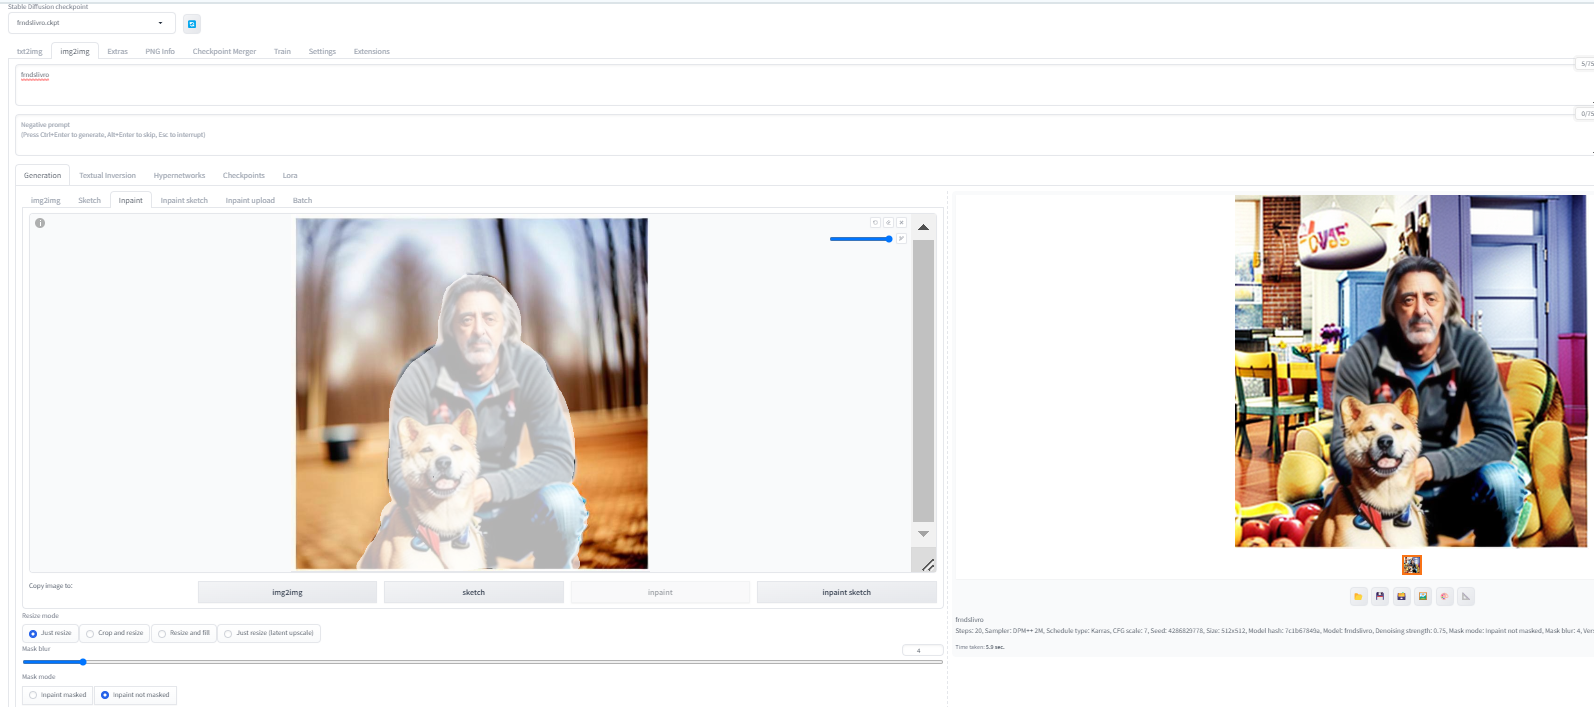
\includegraphics[width = 1
	\textwidth]{Imagenes/Vectorial/inpainting1.png}
	\caption{Ventana de la WEBUI implementada para realizar el painting}
	\label{fig:inpainting1}
\end{figure}

En la figura \ref{fig:inpainting1} se puede ver a la derecha la imagen ``original'', la cual previamente ya había sido pasada por esta técnica para poner la cara de ``80alp'' en la persona anteriormente generada. En la misma figura se puede ver el área \textit{masked} seleccionada con el pincel y el parámetro ``\textit{Mask mode}'' establecido a ``\textit{Inpaint not masked}''. Finalmente, podemos ver en el \textit{prompt} que solamente se especifica el \textit{token} ``frdslivro'' debido a que lo que se quiere conseguir es que sustituya lo que no está seleccionado por la brocha en la imagen, por el salón entrenado del modelo. El resultado puede verse en la parte derecha de la imagen, el cual podemos afirmar que es todo un éxito, al haber conseguido incorporar 3 \textit{tokens} entrenados diferentes, la persona, el animal y el lugar. 

En el siguiente ejemplo de la figura \ref{fig:fasesinpainting} podemos ver la evolución que sigue una misma imagen bajo diferentes peticiones de \textit{prompt} en la fase de \textit{inpainting}. En la primera imagen que se ve en la figura, el \textit{prompt} especificado fue ``a happy 80alp walking with his dog hachift80alp in the forest next to the mountains, day light, full hd, high quality'' y podemos ver como generó todo a la perfección excepto a la persona entrenada. En la segunda foto, se partió de la primera imagen y trazando el área del rostro de la persona, se puso como prompt ``a close up picture of 80alp face, hd''. Finalmente, para que el cuerpo de la persona generada al principio encajara con el de una persona de la edad de la foto, se seleccionó la ropa como área y finalmente el prompt fue ``old man clothes'' y el resultado final fue excepcional. 

\begin{figure}[h]
	\centering
	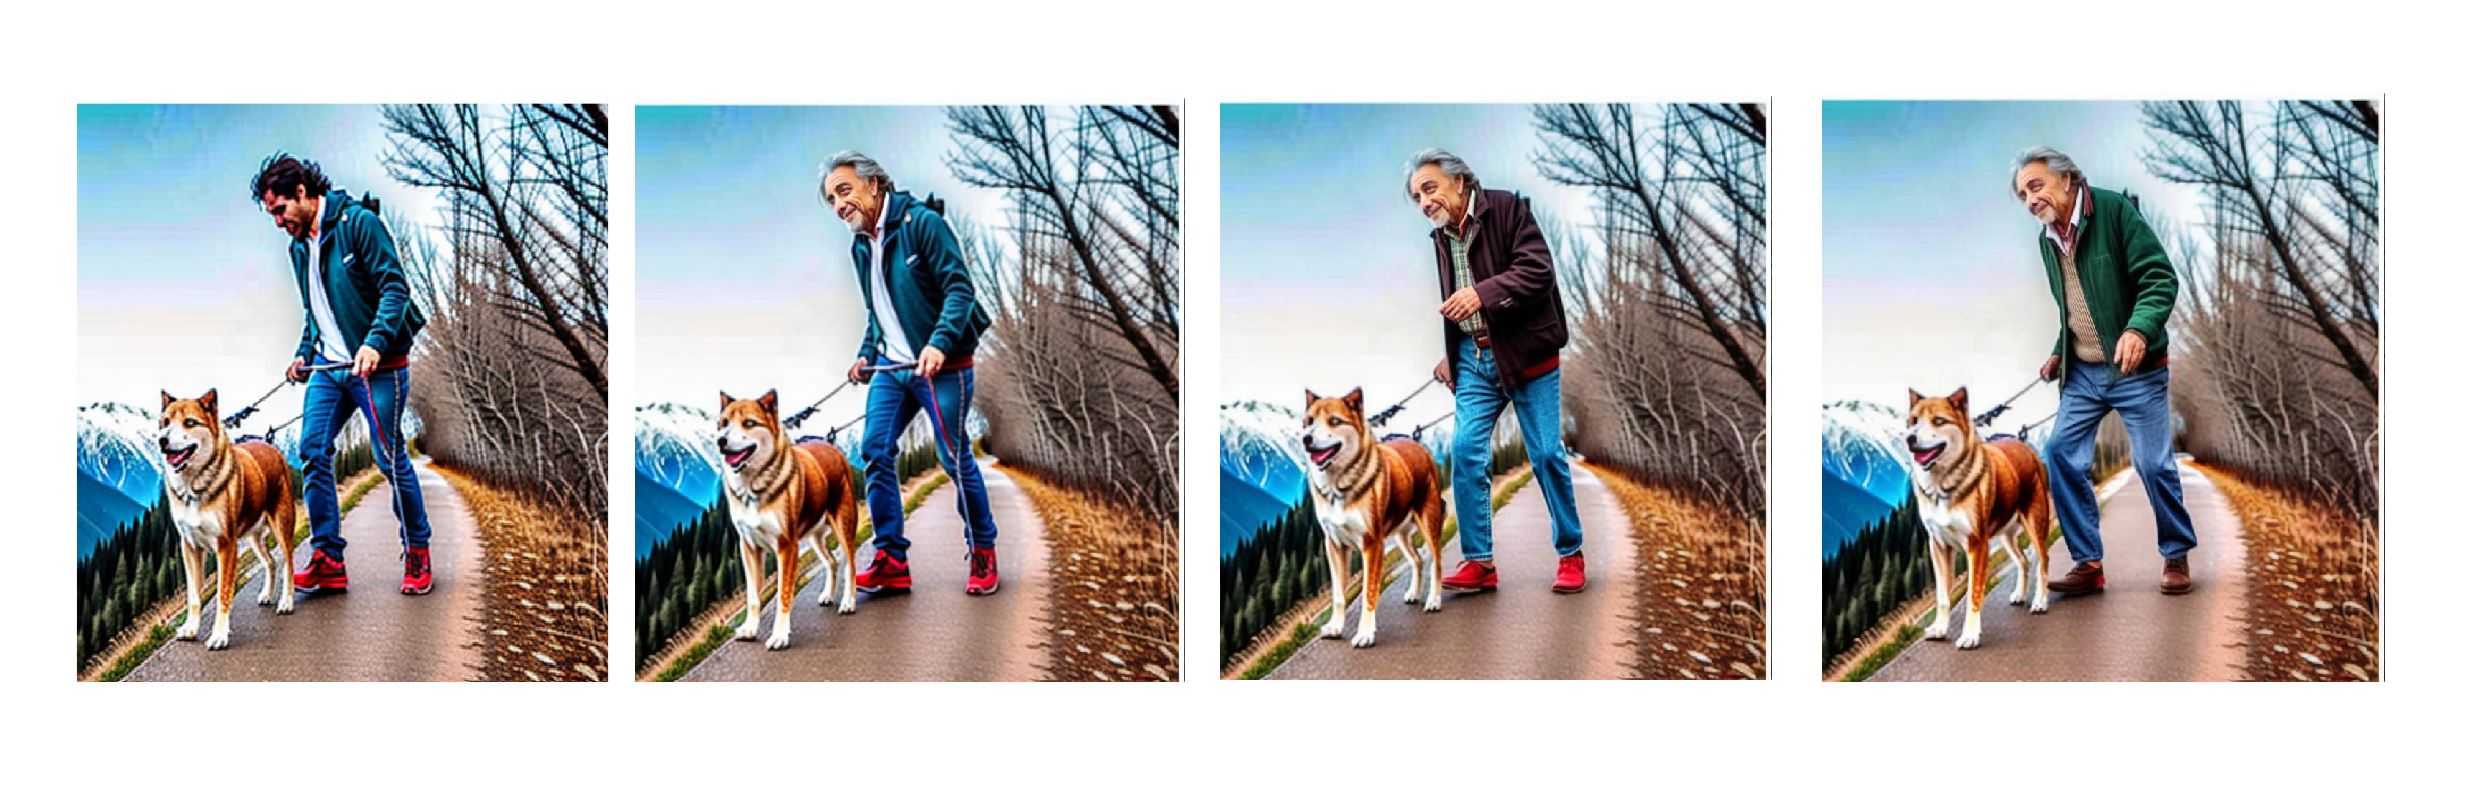
\includegraphics[width = 1.1
	\textwidth]{Imagenes/Vectorial/fasesinpainting.png}
	\caption{Evolución de una imagen con la técnica de inpainting aplicada}
	\label{fig:fasesinpainting}
\end{figure}

\section{Evolución de los modelos del proyecto}

Este apartado muestra los pasos que se han llevado a cabo durante la realización del proyecto. Resulta significativo porque el contraste de lo que se podía hacer al principio con lo que se puede hacer ahora es muy elevado, y pone en valor el trabajo realizado.

1. No se podían generar imágenes en local. No estaba instalado CUDA en el equipo, además de otras herramientas necesarias como Diffusers.

2. Generación de imágenes en local por consola en Anaconda mediante el modelo de Stable Diffusion 1.5. Resultado generado en un archivo. Ejecución lenta y de poca calidad.

3. Generación de imágenes en SDGUI. Buena interfaz que permite la ejecución de imágenes con Stable Diffusion 1.5. Mejor tiempo y calidad. Ya sabemos el modelo más óptimo para desarrollar nuestro proyecto.

4. Se descubre que se pueden utilizar más modelos provenientes de Hugging Face en SDGUI. Se utiliza el Lykon Dreamshaper, basado en LCM, que proporciona alta calidad con muchos menos pasos. No obstante, tiene la limitación de que no se puede personalizar y desarrollar.

5. Intento de generar imágenes personalizadas. Se probarán en SDGUI. Resultados aceptables con LORA. Se puede identificar al elemento entrenado, pero se puede mejorar.

6. Nuevas vías de entrenamiento de modelos. Entrenamiento de Stable Diffusion con Dreambooth. Se identifica el elemento pero se aprecia deformidad.

7. A base de prueba y error, se llega a la conclusión de que el mejor rendimiento se consigue con 2400 pasos de entrenamiento y un dataset de 10 imágenes. Buena calidad en las personas entrenadas, sin deformidad.

8. Se consiguen buenos resultados también en lugares y animales, además de en personas. Se llega a la conclusión de que se puede entrenar cualquier elemento.

9. Se quiere crear una aplicación que utilice esta IA generativa. Al principio se llega a una app con una interfaz poco visual, pero que genera buenas fotografías con el modelo Stable Diffusion 1.5.

10. Versión mejorada de la aplicación, con un backend en Python y un frontend en HTML. Buena interfaz y buenos resultados con modelos pre entrenados, pero no con modelos personalizados.

11. La aplicación ya puede utilizar cualquier modelo entrenado por nosotros mismos. Buenos resultados, con calidad y tiempo comparables a SDGUI.

12. Creación de un libro de vida para la aplicación. Sirve de conexión entre la IA generativa de imágenes desarrollada por nosotros y la creación de historias narrativas con apoyo visual para la terapia de reminiscencia.


